\ac{GP}s are a Bayesian method for regression. We consider the regression input to be real-valued scalars $x_i$ and the regression output as the value of a function $f$ at $x_i$. The complete training data will be denoted by column vectors $\mathbf{x}$ and $\mathbf{f}$. Unseen test data is denoted with $\mathbf{\hat{x}}$ and $\mathbf{\hat{f}}$.
\ac{GP}s present a non-parametric way to express prior knowledge on the space of all possible functions $f$ modeling
a regression relationship.
Formally, a GP is an infinite-dimensional extension of the multivariate Gaussian distribution.

The collection of random variables $\br{f(x)}$ (indexed by $x$) represents the
values of the function $f$ at each location $x$.
We write $f \sim \ac{GP}(m,k)$, where $m$ is the {\em mean function} and $k$ is the {\em covariance function} or {\em kernel}.
That is, $m(x)$ is the prior mean of the random variable $f(x)$, and $k(x,x')$ is the prior covariance of the random variables $f(x)$ and $f(x')$.
Throughout, we write $\mathbf{K}(\xbf,\xbf^\prime)$ for the prior covariance matrix determined by $\xbf$ and $\xbf^\prime$, that is, the covariance between the random vectors $\{f(x)\}_{x \in \xbf}$ and $\{f(x')\}_{x' \in \xbf'}$.
We differentiate three different situations, of how  $f$ can be generated with a \ac{GP}:
\begin{enumerate}
\item $\fbf_*$ - we have not seen any training data yet.
    The \ac{GP} samples at any input vector $\xbf_*$ from the prior with
     $\fbf_* \sim \mathcal{N}\bigg(0,K(\xbf_*,\xbf_*)\bigg)$;
\item $\fbf$ - the observed values for $\fbf:=f(\xbf)$. This is the target value of the value pairs supplied in 
the training data; and
\item $\hat{\fbf}$ - the predictive posterior distribution of test output $\hat\fbf := f(\hat\xbf)$ conditioned on training data $\fbf := f(\xbf)$.
\end{enumerate}We now compute the predictive posterior distribution of test output $\hat\fbf := f(\hat\xbf)$ conditioned on training data $\fbf := f(\xbf)$.  (Here $\xbf$ and $\hat\xbf$ are known constant vectors, and we are conditioning on an observed value of $\fbf$.)  To simplify the calculation, we will assume the prior mean $m$ is identically zero; once the derivation is done, this assumption can be easily relaxed via translation.

The predictive posterior can be computed by first forming the joint density when both training and test data are treated as randomly chosen from the prior, then fixing the value of $\fbf$ to a constant.  To start, let
\[
  \Sigma := \bmat{
    K(\xbf, \xbf)     & K(\xbf, \hat\xbf)     \\
    K(\hat\xbf, \xbf) & K(\hat\xbf, \hat\xbf)
  }
  \text{ and }
  \Sigma^{-1} =: \bmat{
    M_{11} & M_{12} \\
    M_{21} & M_{22}
  }.
\]
We then have
\[
  P(\fbf, \hat\fbf)
  \propto
  \exp\br{
    -\frac12
    \bmat{\fbf^\top & \hat\fbf^\top}
    \bmat{M_{11} & M_{12} \\ M_{21} & M_{22}}
    \bmat{\fbf \\ \hat\fbf}
  }.
\]
Treating $\fbf$ as a fixed constant, we obtain
\[
  P\pn{\hat\fbf \mvert \fbf}
  \propto
  P(\fbf, \hat\fbf)
  \propto
  \exp\br{
    -\frac12 \hat\fbf^\top M_{22} \hat\fbf
    - \hbf^\top \hat\fbf
  },
\]
where $\hbf = M_{21} \fbf$ is a constant vector.  Thus $P(\hat\fbf | \fbf)$ is Gaussian,
\begin{equation}\label{eq:pred_posterior}
  P\pn{\hat\fbf \mvert \fbf} \sim \Ncal(\hat\mubf, \hat\Kbf),
\end{equation}
with covariance matrix $\hat\Kbf = M_{22}^{-1}$.  To find its mean $\hat\mubf$, we note that $P_{\hat\fbf|\fbf}(\hat\fbf + \hat\mubf)$ is Gaussian with the same covariance as $P(\hat\fbf | \fbf)$, but its exponent has no linear term:
\begin{align*}
  P_{\hat\fbf|\fbf} \pn{\hat\fbf + \hat\mubf \mvert \fbf}
  &\propto
  \exp\br{
    -\frac12 (\hat\fbf + \hat\mubf)^\top M_{22} (\hat\fbf + \hat\mubf)
    - \hbf^\top (\hat\fbf + \hat\mubf)
  } \\
  &\propto
  \exp\br{
    -\frac12 \hat\fbf^\top M_{22} \hat\fbf
    - \underbrace{(\hbf + M_{22} \hat\mubf)^\top}_{\text{must be $0$}} \hat\fbf
  }.
\end{align*}
Thus $\hbf = -M_{22} \hat\mubf$ and $\hat\mubf = -M_{22}^{-1} \hbf = -M_{22}^{-1} M_{21} \fbf$.

The partioned inverse equations (\citealp*{barnett1979matrix} following \citealp*{mackay1998introduction}) give
\begin{align*}
  M_{22}^{-1} &= K(\hat\xbf,\hat\xbf) - K(\hat\xbf,\xbf) K(\xbf,\xbf)^{-1} K(\xbf,\hat\xbf), \\
  M_{21} &= -M_{22} K(\hat\xbf,\xbf) K(\xbf,\xbf)^{-1}.
\end{align*}
Substituting these in the above gives
\begin{align}
  \hat\Kbf &= K(\hat\xbf,\hat\xbf) - K(\hat\xbf,\xbf) K(\xbf,\xbf)^{-1} K(\xbf,\hat\xbf),\label{eq:K_hat} \\
  \hat\mubf &= K(\hat\xbf,\xbf) K(\xbf,\xbf)^{-1}\fbf.\label{eq:mu_hat}
\end{align}
Together, $\hat\mubf$ and $\hat\Kbf$ determine the computation of the predictive posterior
with unseen input data (\ref{eq:pred_posterior}).

Often one assumes the observed regression output is noisily measured, that is, one only sees the values of $\ybf_\noisy = \mathbf{f}+ \wbf$ where $\wbf$ is Gaussian white noise with variance $\sigma_\noise^2$. This noise term can be absorbed into the covariance matrix $\mathbf{K}(\mathbf{x},\mathbf{x})$ which in the following, we will write as $\mathbf{K}$ for readability. The log-likelihood of a \ac{GP} can then be written as:
\begin{equation}
\label{eq:gplogdens}
\log P(\mathbf{f} \mid \xbf) =
-\frac12 \ybf^\top 
\mathbf{K}^{-1} \ybf
- \frac12\log \abs{\mathbf{K}}
- \frac{n}{2}\log 2\pi
\end{equation}
where $n$ is the number of data points.
Both log-likelihood and predictive posterior can be computed efficiently using a \ac{SP} in Venture~\citep{mansinghka2014venture}
with an algorithm that resorts to Cholesky factorization\citep[chap. 2]{rasmussen2006gaussian}. 
We write the Cholesky factorization as 
$\mathbf{L} \coloneqq \text{chol}(\mathbf{K})$ when
:
\begin{equation}
\mathbf{K} = LL^\top
\end{equation}
where L is a lower triangular matrix. This allows us to compute the inverse of a covariance matrix as
\begin{equation}
\mathbf{K}^{-1} = (\mathbf{L}^{-1})^\top (\mathbf{L}^{-1})
\end{equation}
and its determinant as 
\begin{equation}
det(\mathbf{K}) = det(\mathbf{L})^2
\end{equation}
We compute (\ref{eq:gplogdens}) as
\begin{equation}
\log(P(\mathbf{f}\mid \mathbf{x})\coloneqq - \frac{1}{2} \mathbf{f}^\top \bm{\alpha} - \sum_i \log \mathbf{L}_{ii} - \frac{n}{2} \log 2 \pi
\end{equation}
where 
\begin{equation}
\label{eq:chol_L}
\mathbf{L} \coloneqq \text{chol}(\mathbf{K})
\end{equation}
and 
\begin{equation}
\label{eq:alpha}
\bm{\alpha} \coloneqq  \mathbf{L}^\top \backslash(\mathbf{L} \backslash \mathbf{f}). 
\end{equation}
%This results in a computational complexity of $\mathcal{O}(n^3)$ in the number of data points for
%sampling with a complexity of $n^3/6$ for (\ref{eq:chol_L}) an $n^2/2$ for (\ref{eq:alpha}). 
This results in a computational complexity for sampling in the number of data points of $O(n^3/6)$ for (\ref{eq:chol_L}) an $O(n^2/2)$ for (\ref{eq:alpha}). 
%%%%%%%%%%%%%%%%%%%%%%%%%%%%%%%%%%%%%%%%%%%%%%%%%%%%%%%%%%%%
%%%%%%%%%%%%%%%%%%%%%%%%%%%%%%%%%%%%%%%%%%%%%%%%%%%%%%%%%%%%
%%%%%%%%%%%%%%%%%%%%%%%%%%%%%%%%%%%%%%%%%%%%%%%%%%%%%%%%%%%%
\subsection{Covariance Functions}
The covariance function (or kernel) of a \ac{GP} governs high-level properties of the observed data such as linearity, periodicity and smoothness.
It comes with few free parameters that we call hyper-parameters.
Adjusting the hyper-parameters changes non-qualitative attributes such as length
scales while preserving the qualitative properties of the distribution.
These high-level properties are compositional via addition and multiplication of different covariance functions. An addition models a global interaction, that is an interaction of two high-level components that is qualitatively not dependent on the input space. An example for this a periodic function with a linear trend.
A multiplication models a local interaction of two components. 
An example for this is a periodic function with a linearly increasing amplitude. We demonstrate kernel composition with local interactions in the tutorial in Fig. \ref{fig:composition_tutorial}. 


\begin{figure}
 \centering

     \begin{subfigure}[b]{0.45\textwidth}
        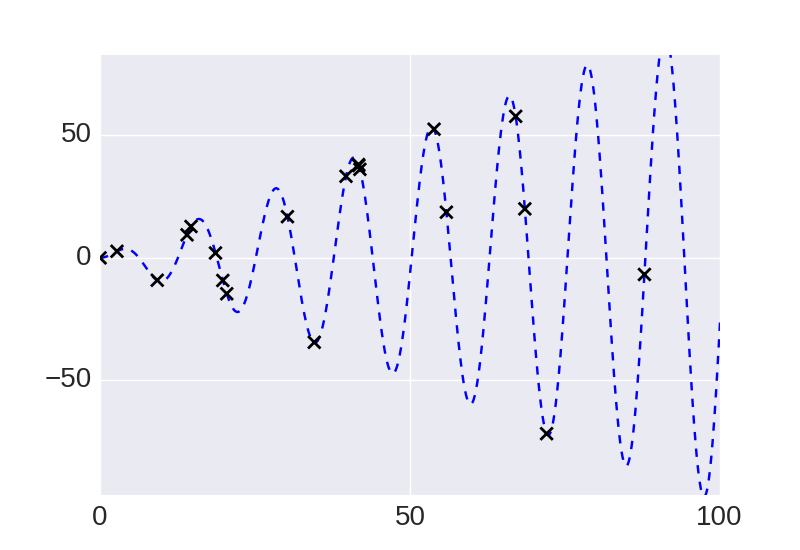
\includegraphics[width=\textwidth]{figs/composition/composition_demo_raw_data.png}
        \caption{Raw Data}
    \end{subfigure}
    ~ %add desired spacing between images, e. g. ~, \quad, \qquad, \hfill etc. 
      %(or a blank line to force the subfigure onto a new line)
    \begin{subfigure}[b]{0.45\textwidth}
\small
     \begin{align*}
    \text{LIN} &=   \sigma_1^2(x x^\prime)\\
    \text{PER} &=  \sigma_2^2 \exp \bigg( \frac{2 \sin^2 ( \pi (x - x^\prime)/p}{\ell^2} \bigg)\\ 
    \text{LIN} \times \text{PER} &=  \sigma_1^2(x x^\prime)\, \sigma_2^2 \exp \bigg( \frac{2 \sin^2 ( \pi (x - x^\prime)/p}{\ell^2} \bigg) 
    \end{align*}\vspace{5mm} 
        \caption{Kernels}
    \end{subfigure}\vspace{4mm} 


Parameterized Kernels:\vspace{3mm} 

     \begin{subfigure}[b]{0.3\textwidth}
      \centering \footnotesize
       $20.1^2(x x^\prime) $ \vspace{2mm}
	\caption{LIN}
    \end{subfigure}
    ~ %add desired spacing between images, e. g. ~, \quad, \qquad, \hfill etc. 
      %(or a blank line to force the subfigure onto a new line)
    \begin{subfigure}[b]{0.3\textwidth}
      \centering \footnotesize
      $19.1^2 \exp \bigg( \frac{2 \sin^2 ( \pi (x - x^\prime)/37.7}{6.3^2} \bigg)$ 
	\caption{PER}
    \end{subfigure}
    ~ %add desired spacing between images, e. g. ~, \quad, \qquad, \hfill etc. 
    %(or a blank line to force the subfigure onto a new line)
    \begin{subfigure}[b]{0.3\textwidth}
    \centering \footnotesize
      $383.9^2 (x x^\prime) \exp \bigg( \frac{2 \sin^2 ( \pi (x - x^\prime)/37.7}{6.3^2} \bigg)$ 
        \caption{LIN $\times$ PER}
    \end{subfigure} \vspace{4mm} 

Prior:

     \begin{subfigure}[b]{0.3\textwidth}
        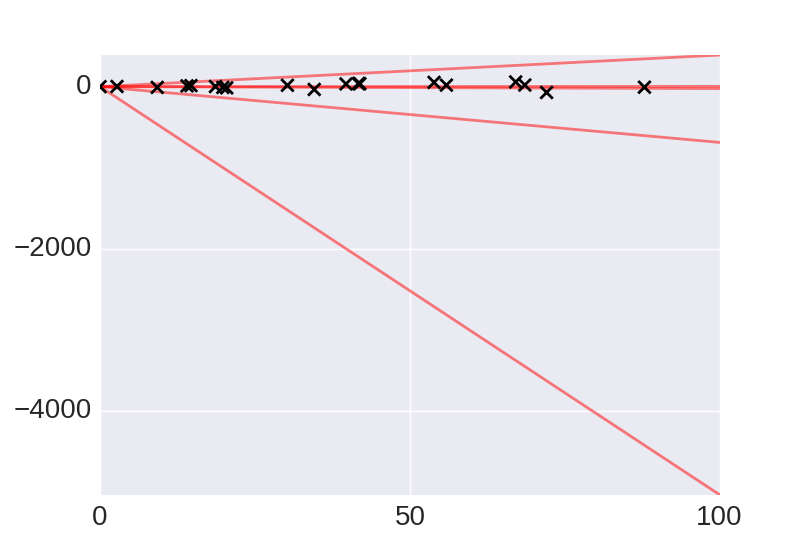
\includegraphics[width=\textwidth]{figs/composition/composition_demo_LIN_prior.png}
        \caption{LIN}
    \end{subfigure}
    ~ %add desired spacing between images, e. g. ~, \quad, \qquad, \hfill etc. 
      %(or a blank line to force the subfigure onto a new line)
    \begin{subfigure}[b]{0.3\textwidth}
        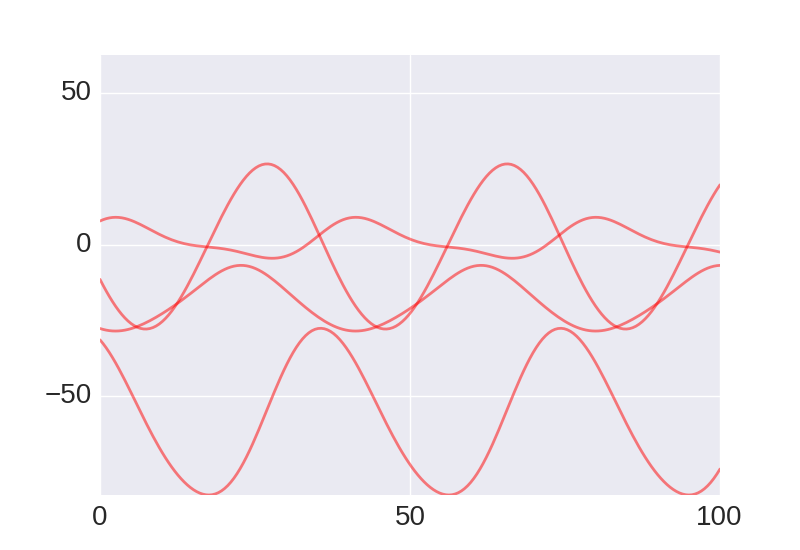
\includegraphics[width=\textwidth]{figs/composition/composition_demo_PER_prior.png}
        \caption{PER}
    \end{subfigure}
    ~ %add desired spacing between images, e. g. ~, \quad, \qquad, \hfill etc. 
    %(or a blank line to force the subfigure onto a new line)
    \begin{subfigure}[b]{0.3\textwidth}
        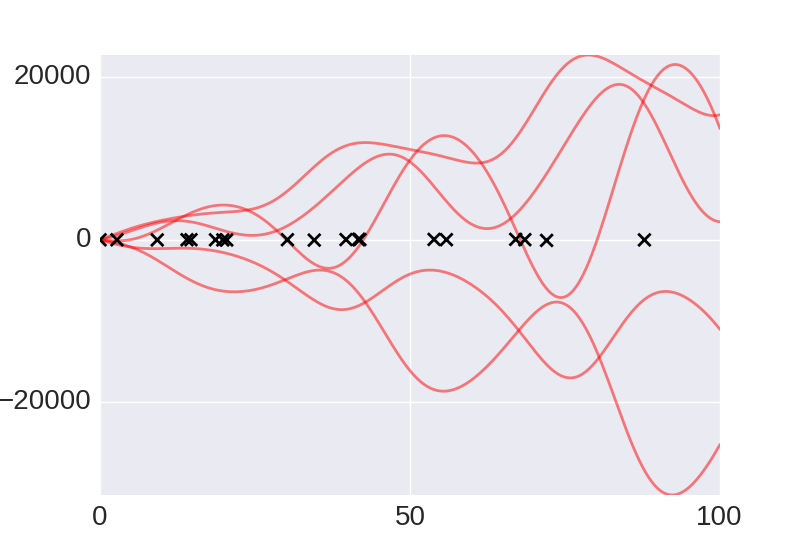
\includegraphics[width=\textwidth]{figs/composition/composition_demo_LINxPER_prior.png}
        \caption{LIN $\times$ PER}
    \end{subfigure} \vspace{4mm} 

Posterior:

 \begin{subfigure}[b]{0.3\textwidth}
        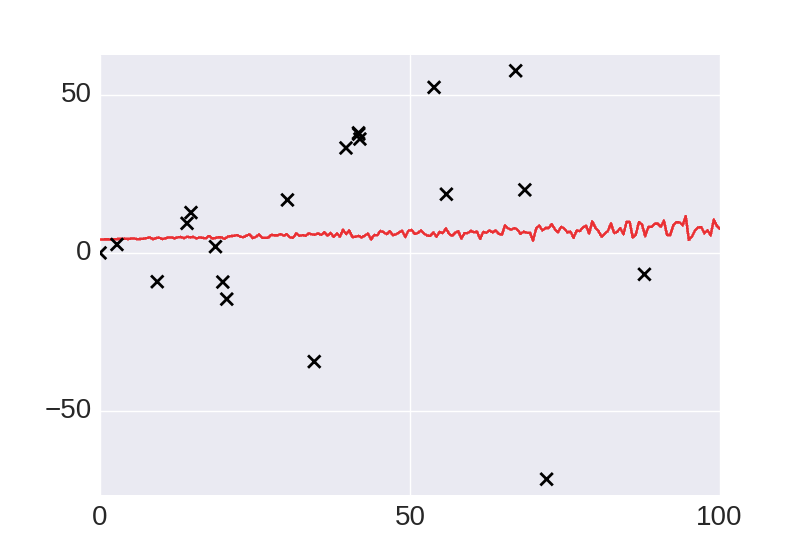
\includegraphics[width=\textwidth]{figs/composition/composition_demo_LIN.png}
        \caption{LIN}
    \end{subfigure}
    ~ %add desired spacing between images, e. g. ~, \quad, \qquad, \hfill etc. 
      %(or a blank line to force the subfigure onto a new line)
    \begin{subfigure}[b]{0.3\textwidth}
        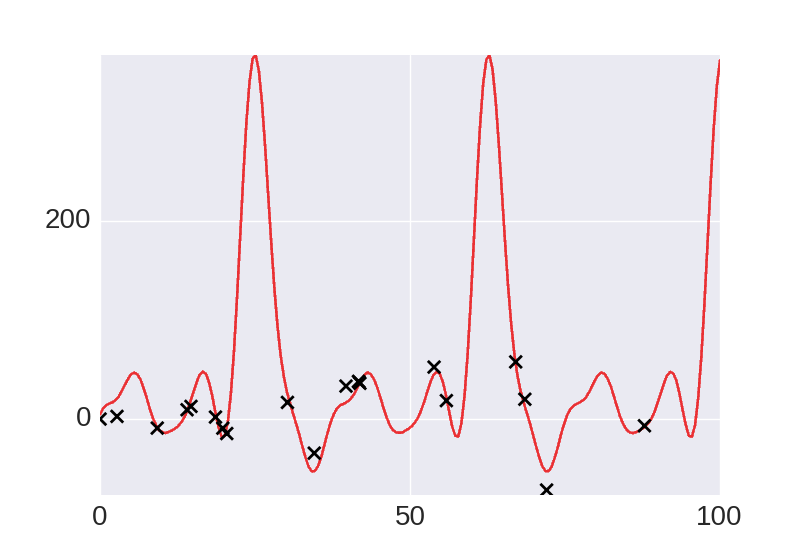
\includegraphics[width=\textwidth]{figs/composition/composition_demo_PER.png}
        \caption{PER}
    \end{subfigure}
    ~ %add desired spacing between images, e. g. ~, \quad, \qquad, \hfill etc. 
    %(or a blank line to force the subfigure onto a new line)
    \begin{subfigure}[b]{0.3\textwidth}
        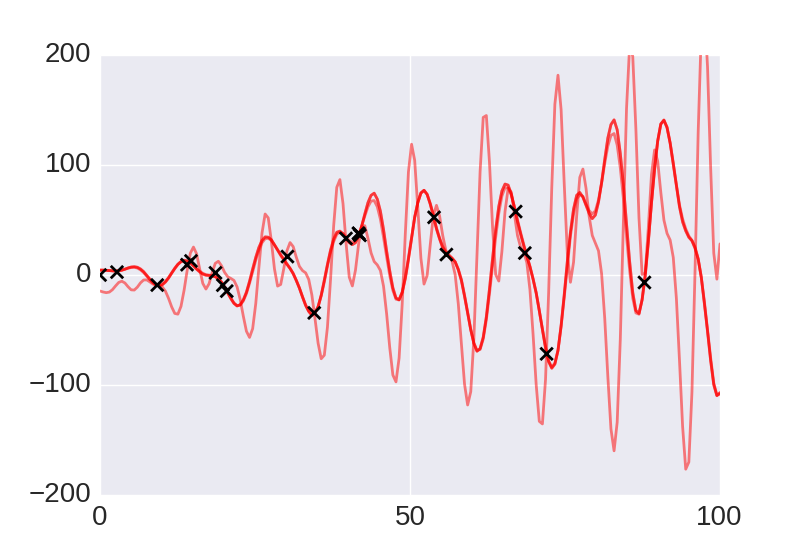
\includegraphics[width=\textwidth]{figs/composition/composition_demo_LINxPER.png}
        \caption{LIN $\times$ PER}
    \end{subfigure}

%20.0739791735
%6.31647597198
%37.7184218042
%19.1051376016

\caption{We depict kernel composition. 
(a) shows raw data (black) generated with a sine function with linearly growing amplitude (blue). 
(b) shows the linear and the periodic base kernel as well as a composition of both. 
The multiplication of the two kernels indicates local interaction. The local interaction we account for in this case is the growing amplitude (a). (c-e) show the parameterized kernels that we introduced in (b).
The parameters are sampled from the posterior distribution on parameters for a \ac{GP} with kernel $\mathbf{K}=\text{LIN} \times \text{PER}$ where the data points from (a) are observed.
(f-h) show samples from the prior where the parametrization from (c-e) is used, that is, before any data points are observed.
(i-k) show samples from the posterior, after the data has been observed. Note that the same data is used for all of the plots.}
\label{fig:composition_tutorial}
\end{figure}

